% diagrams/english/clase.tex -- la clase de Marta, para "Where is it?":
% la pizarra, la mesa de la maestra (con cajones y sitio debajo), el
% reloj de la pared y la puerta. Se dibujan encima las cosas que dice
% el texto.
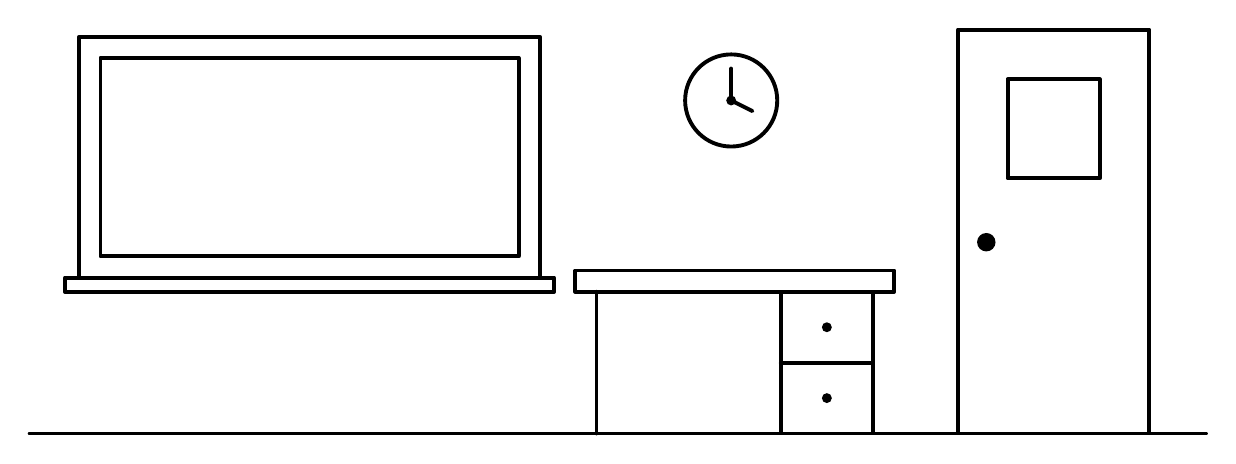
\begin{tikzpicture}[line width=1.4pt, line cap=round, line join=round, scale=0.9]
  \draw (-0.3,0) -- (16.3,0);
  % la pizarra, con su marco y la repisa de las tizas
  \filldraw[fill=white] (0.4,2.2) rectangle (6.9,5.6);
  \draw (0.7,2.5) rectangle (6.6,5.3);
  \filldraw[fill=white] (0.2,2.0) rectangle (7.1,2.2);
  % el reloj
  \filldraw[fill=white] (9.6,4.7) circle (0.65);
  \draw (9.6,4.7) -- (9.6,5.15); \draw (9.6,4.7) -- (9.9,4.55);
  \fill (9.6,4.7) circle (0.07);
  % la mesa de Marta, con los cajones a la derecha (y sitio debajo, a la
  % izquierda)
  \filldraw[fill=white] (7.4,2.0) rectangle (11.9,2.3);
  \draw (7.7,2.0) -- (7.7,0);
  \filldraw[fill=white] (10.3,0) rectangle (11.6,2.0);
  \draw (10.3,1.0) -- (11.6,1.0);
  \fill (10.95,1.5) circle (0.07); \fill (10.95,0.5) circle (0.07);
  % la puerta, con su ventanita y el pomo
  \filldraw[fill=white] (12.8,0) rectangle (15.5,5.7);
  \draw (13.5,3.6) rectangle (14.8,5.0);
  \fill (13.2,2.7) circle (0.13);
\end{tikzpicture}
